% =========================================================================
% Sensitivity-Aware Static Placement for All-Analog GPT-2 Inference
% on Heterogeneous, Aging In-Memory Compute Tiles
%
% Target: IEEE Computer Architecture Letters (journal option of IEEEtran).
% Compile on Overleaf (pdfLaTeX). Figures live in figures/.
% =========================================================================
\documentclass[journal]{IEEEtran}

\usepackage{graphicx}
\usepackage{amsmath,amssymb}
\usepackage{booktabs}
\usepackage[caption=false,font=footnotesize]{subfig}
\renewcommand{\arraystretch}{0.92}
\setlength{\textfloatsep}{5pt plus 1pt minus 2pt}
\setlength{\floatsep}{5pt plus 1pt minus 1pt}
\setlength{\abovecaptionskip}{3pt}
\usepackage[hidelinks]{hyperref}

\newcommand{\policy}[1]{\texttt{#1}}
\newcommand{\dnll}{\Delta\mathrm{NLL}}

\begin{document}

\title{Sensitivity-Aware Static Placement Sustains All-Analog GPT-2
Inference on Heterogeneous, Aging In-Memory Compute Tiles}

\author{Wei~Ju~Hwang%
\thanks{W.~J.~Hwang is with the University of Toronto, Toronto, ON,
Canada (e-mail: william.ju@mail.utoronto.ca).}%
\thanks{Manuscript received XXXX; revised XXXX.}}

\markboth{IEEE Computer Architecture Letters}%
{Hwang: Sensitivity-Aware Static Placement for All-Analog GPT-2 Inference}

\maketitle

% -------------------------------------------------------------------------
\begin{abstract}
Analog in-memory computing (AIMC) tiles are heterogeneous at fabrication
and degrade unevenly in the field, yet the assignment of weight blocks to
physical tiles---\emph{placement}---is free at map time. We study whether
this free decision determines deployment quality for a decoder-only
language model executed \emph{entirely} on analog tiles. A five-phase pipeline
combines hardware-aware fine-tuning of GPT-2 with a measured
per-projection sensitivity profile and static shard placement onto a
simulated $96{\times}8$ substrate whose tile noise drifts, fluctuates,
and suffers faults over a 120-step aging trace. On the full WikiText-103 test set, across five
independent hardware traces, sensitivity-aware placement maintains a
$+0.063$-nat advantage over the strongest workload-blind baseline (95\% t-CI
$[0.042, 0.084]$, 5/5 traces) and keeps perplexity below the digital
reference in all 75 evaluated conditions, whereas every baseline
crosses above digital in some end-of-life conditions. Bounding
experiments show the one-shot $t{=}0$ placement captures 97.8\% of the
achievable headroom and is statistically indistinguishable from a
clairvoyant placement that knows the entire degradation trajectory; a
six-scenario parameter sweep finds the benefit positive in 48/48 paired
conditions and monotone in tile-quality spread. Placement, not just noise
tolerance, decides whether an all-analog LLM deployment remains worth
using over its lifetime.
\end{abstract}

\begin{IEEEkeywords}
Analog in-memory computing, weight mapping, placement, large language
models, hardware-aware training, reliability.
\end{IEEEkeywords}

% -------------------------------------------------------------------------
\section{Introduction}
\IEEEPARstart{A}{nalog} in-memory computing executes matrix--vector
products inside memory crossbars, promising large energy and latency
gains for DNN inference at the cost of storing weights as noisy
conductances~\cite{joshi2020,rasch2023}. Real substrates are
\emph{heterogeneous} and \emph{non-stationary}: programming-noise spread
across tiles, conductance drift, spatially correlated thermal variation,
and localized permanent faults are all documented at
scale~\cite{joshi2020,legallo2018,wan2022}. A deployment must therefore
decide which weight block lives on which physical tile. This choice costs
nothing at map time, but tiles differ in quality---and age differently.

Existing heterogeneous-mapping work optimizes a different axis: which
operations stay \emph{digital}. Layer-, channel-, and weight-granular
methods partition workloads across analog tiles and digital compute
units~\cite{lionheart,mps}, leaving the intra-analog assignment
unspecified---in practice it defaults to the sequential or random
orders we use as baselines. A complementary line remaps weights around
stuck-at faults and steers significant weights toward reliable cells
\emph{within} a crossbar~\cite{xia2018,zhang2019}---CNN-scale,
single-snapshot, often with retraining; tile-granular quality
differences of an aging substrate remain unaddressed. A recent letter
distills the partitioning methods into a unified workflow and contributes the first AIMC precision-sensitivity
profile of a decoder-only transformer~\cite{lammie2026}; it
leaves two questions open: whether time-dependent degradation invalidates
static mappings, and how mapping should exploit intra-analog tile-quality
differences. We answer both for a fully analog deployment: \emph{no
digital fallback}, with placement as the only degree of freedom.

\textbf{Contributions.}
(i)~An end-to-end pipeline that makes pretrained GPT-2 functional
under a documented analog noise contract and evaluates placement on the
full WikiText-103 test set under a time-resolved aging model.
(ii)~A paired, multi-seed statistical design: five independent hardware
traces are the units of inference; identical Gaussian coordinate fields
across policies remove realization variance from every comparison.
(iii)~Evidence that sensitivity-aware static placement keeps the
deployment better than its digital reference over the entire simulated
lifetime while every workload-blind policy fails this test.
(iv)~Placement \emph{bounds}: an adversarial worst case and a
clairvoyant trajectory-aware reference showing the one-shot policy is
near-optimal.

% -------------------------------------------------------------------------
\section{All-Analog Deployment Pipeline}
\label{sec:pipeline}

The pipeline has five phases sharing one frozen configuration and one
noise contract; only the hardware-trace seed varies between runs. All
experiments use GPT-2 Small (124M)~\cite{gpt2} and
WikiText-103~\cite{wikitext} (train split for fine-tuning, validation for
calibration, held-out test for all reported quality numbers), simulated
with IBM's AIHWKit~\cite{aihwkit,legallo2023}.
Fig.~\ref{fig:workflow} situates the contribution: Phases~0--1 supply
the mapper's inputs, the mapper drops into the standard flow's mapping
stage, and Phase~2's role is played in deployment by per-chip
calibration.

\begin{figure}[t]
\centering
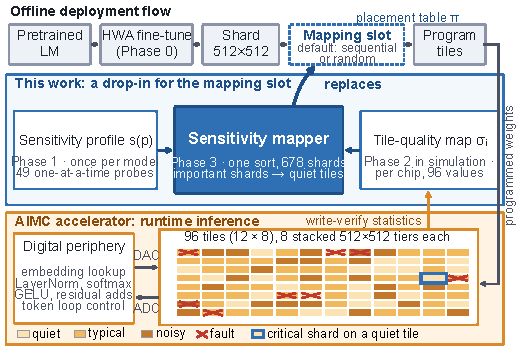
\includegraphics[width=0.85\columnwidth]{figures/workflow.pdf}
\caption{Where the contribution sits in an LLM-on-CIM deployment: a
drop-in for the mapping stage, consuming a one-off model sensitivity
profile and a per-chip calibrated tile-quality map, emitting the
shard-to-tile placement table---nothing else changes, zero runtime
hardware. Shading encodes tile noise.}
\label{fig:workflow}
\end{figure}

\subsection{Noise Contract}
Every analog projection is clipped once at $2.5\sigma$ of its weight
distribution (symmetric about zero, matching differential-pair
conductance ranges), tiled into $512{\times}512$ crossbar shards, and
converted with ${\sim}8$-bit ADC/DAC. Additive Gaussian weight noise is
expressed as a normalized standard deviation---a fraction of the
projection's programmed (peak-to-peak) range---with deployment reference
$\sigma_{\mathrm{ref}}{=}0.023$, calibrated to measured PCM programming
noise at ${\approx}4$-bit effective precision~\cite{joshi2020,legallo2023}.
AIHWKit's internal noise sources are disabled: the contract above is the
\emph{only} noise in the simulation. This configuration coincides setting-for-setting with the one IBM
published for its GPT-2 AIMC study~\cite{lammie2026}, chosen
independently from the same measurements.

\subsection{Phase 0: Hardware-Aware Fine-Tuning}
Post-training conversion of pretrained GPT-2 to this contract is
non-functional (perplexity $29 \rightarrow \approx 3{,}146$ before any
tile noise). We therefore fine-tune for 2{,}000 steps with
perturb-forward/clean-update noise injection~\cite{joshi2020,rasch2023}:
each forward pass clips via a straight-through estimator~\cite{ste} and
perturbs every projection with
$\sigma \sim \mathcal{U}(0, 2\sigma_{\mathrm{ref}})$, covering the
substrate's full class-multiplier range at deployment. The tied LM head is noised
only in its matmul role, exactly as deployed.

\subsection{Phase 1: Measured Sensitivity Profile}
For each of the 49 projections $p$ (48 transformer projections + LM
head), one projection at a time is made analog while the rest stay
digital, and
\begin{equation}
s(p) = \mathbb{E}_r\!\left[\,\mathrm{NLL}\big(W^{c}_p + \sigma_{\mathrm{ref}}
R_p Z_r\big)\right] - \mathrm{NLL}_{\mathrm{ref}}(p),
\end{equation}
with $R_p$ the programmed range, five antithetic noise pairs $Z_r$, and
$\mathrm{NLL}_{\mathrm{ref}}(p)$ that projection's clipped, quantized,
zero-noise reference (isolating noise from conversion effects). The profile is strongly structured
(Fig.~\ref{fig:ranking}): the LM head ($0.061$ nats) and block~0's
attention output ($0.034$) dominate, with a rank-1-to-rank-49 spread of
${\sim}540\times$, and the ordering matches the
pretrained model's profile at ${\sim}100\times$ larger magnitudes---the
structure is architectural and survives hardware-aware training,
corroborating the pretrained-model profile of~\cite{lammie2026};
weight magnitude, the obvious free proxy, is uncorrelated with the
measured profile (Spearman $\rho=-0.08$). The profile costs 540
forward passes over the 250k-token calibration split, once per
model---not per chip.

\begin{figure}[t]
\centering
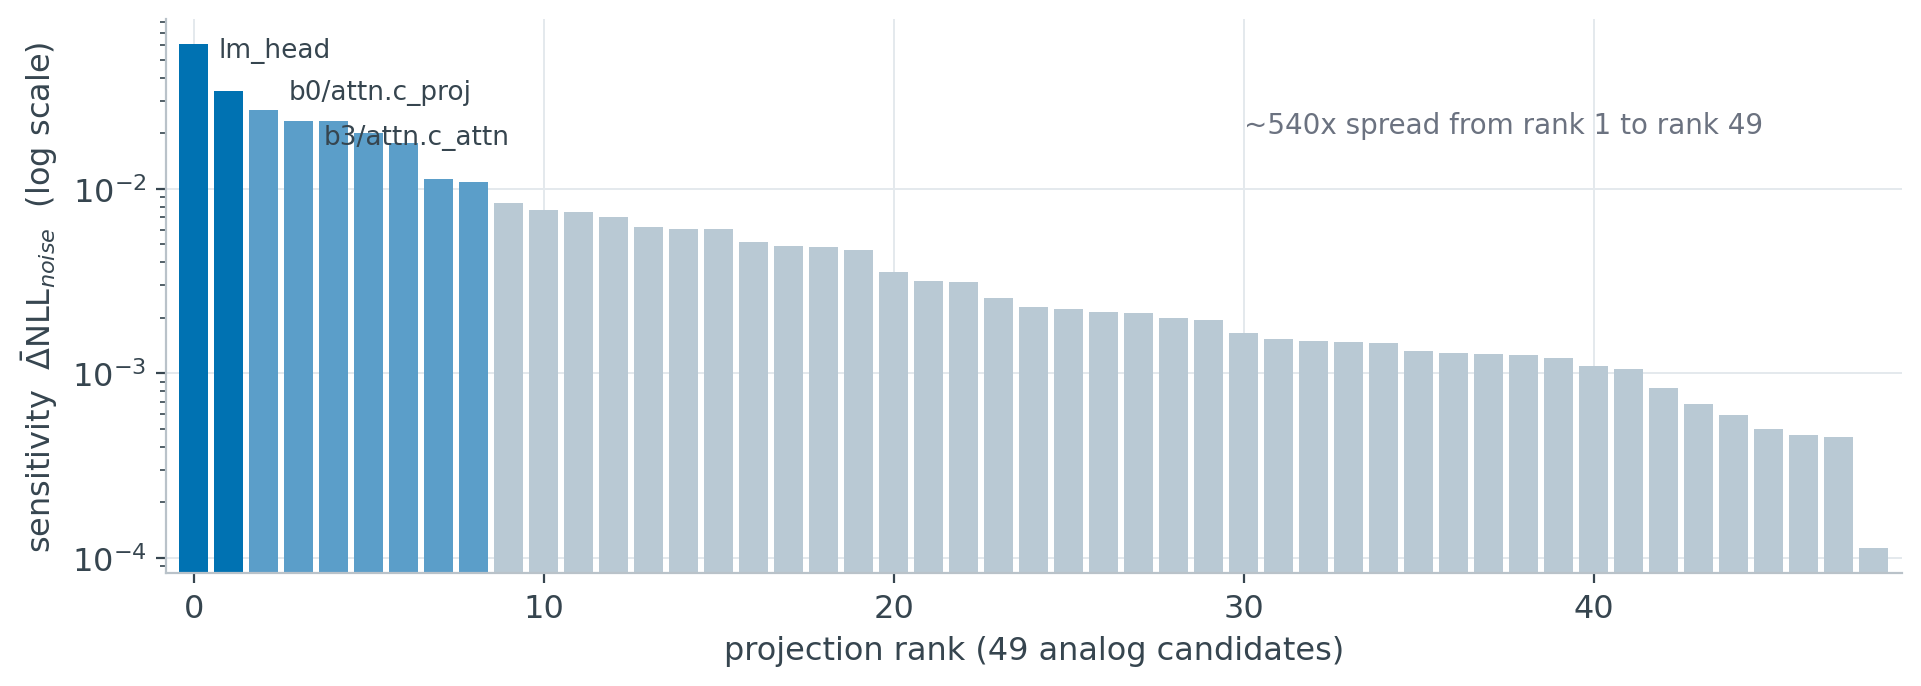
\includegraphics[width=0.84\columnwidth]{figures/p1_ranking.png}
\caption{Measured post-HWA sensitivity of all 49 GPT-2 projections at
$\sigma_{\mathrm{ref}}{=}0.023$ (log scale; five antithetic noise
pairs). The LM head and
early-block attention outputs dominate by orders of magnitude---the
spread placement exploits.}
\label{fig:ranking}
\end{figure}

\subsection{Phase 2: Time-Varying Tile Fidelity}
The substrate has 96 tiles $\times$ 8 tiers of $512{\times}512$
crossbars. Tile $i$'s normalized noise at timestep $t \in [0, 119]$ is
\begin{equation}
\sigma_i(t) = b_i\,\big(d_i(t) + H_{z(i)}(t)\big)\cdot f_i(t),
\end{equation}
where $b_i = \sigma_{\mathrm{ref}} m_i$ with class multipliers $m_i$
drawn from a 25/50/25\% healthy/typical/poor taxonomy
($0.65$--$1.70\times$, spanning reported array-to-array
spread~\cite{joshi2020}); $d_i(t)$ ramps $+12$--$35\%$
over the window (PCM drift exponents $\nu \approx
0.03$--$0.1$~\cite{legallo2018}); $H_z$ is zone-correlated AR(1)
variation ($\rho = 0.94$, 8 zones)~\cite{wan2022}; and $f_i(t)$ steps
permanently from $1$ to $1.25$--$1.70$ on 8 tiles at onsets $t \sim
\mathcal{U}(35, 90)$~\cite{wan2022}. Values are scenario parameters
motivated by these measurements, not calibrated to one device; timesteps
are dimensionless. Section~\ref{sec:sweep} shows the conclusions do not
depend on these choices.

\subsection{Phase 3: Sharding and Placement Policies}
The 49 projections tile into 678 shards (fused Q/K/V region boundaries
are never crossed), each assigned to one of 768 physical tiers. Shard
importance is $I_s = \max(s(p), 0)\,|W_s|/|W_p|$, and placements are
compared at map time by the separable diagnostic
$\Phi = \sum_s I_s\,\sigma^2_{\mathrm{tile}(s)}$.
Policies: \policy{random} (seeded shuffle); \policy{sequential} (slot
order); \policy{hardware\_only} (quietest tiles first, shard order
random---workload-blind but hardware-aware, the strongest fair baseline);
and \policy{static\_sensitivity} (quietest tiles first, most important
shards first), which is provably $\Phi$-optimal at $t{=}0$ by the
rearrangement inequality. The 90 spare tiers let quality-sorted policies leave the worst
capacity empty; \policy{hardware\_only} shares this advantage, so its
gap isolates importance ordering specifically. The mapper itself is one
sort over the 678 shards---negligible map-time compute, zero runtime
cost. Two bounds complete the span:
\policy{adversarial} (most important shards onto the noisiest tiles) and
\policy{oracle\_clairvoyant}, the same sorted rule applied to the
\emph{trajectory-RMS} noise
$\bar{\sigma}_i = (\tfrac{1}{T}\sum_t \sigma_i^2(t))^{1/2}$---a
reference that knows every future fault and drift rate at map time. All placements are static.

% -------------------------------------------------------------------------
\section{Evaluation Protocol}
\label{sec:protocol}

For each policy, timestep $t \in \{0, 30, 60, 90, 119\}$, and
realization $r \in \{1,2,3\}$, tile noise is materialized once into the
logical weights,
\begin{equation}
W^{\mathrm{noisy}}[s] = W_c[s] + \sigma_{\mathrm{tile}(s)}(t)\, R_p\,
Z_{p,r}[s],
\end{equation}
and the full test set (285{,}417 predicted tokens) is evaluated through
the AIHWKit analog forward path. The standard-normal field $Z_{p,r}$ is
keyed by projection and realization only---\emph{policies see identical
noise coordinates and differ solely through tile scales}---so paired
policy differences are free of realization variance; seeded policy orders vary per trace. Two references are
measured once per trace: the \emph{digital} model (plain forward,
$\mathrm{PPL} = 42.91$) and the \emph{nominal} all-analog model (clip +
quantization, zero tile noise). Quality is token-weighted NLL
(nats/token); perplexity is reported for intuition only, since paired
$\dnll$ differences are level-independent ($\dnll \approx$ relative
PPL change) and t-based intervals are computed on the NLL scale. The 15
within-trace samples share one correlated trajectory, so
\emph{inference uses the five independent traces (seeds 41--45) as
statistical units}.

% -------------------------------------------------------------------------
\section{Results}

\subsection{The All-Analog Deployment Is Functional}
\label{sec:r1}
The hardware-aware model is native to the clipped, quantized regime: its
nominal all-analog perplexity is $31.50$ versus $42.91$ for its own
unclipped digital evaluation. This inversion is expected, not anomalous:
Phase~0 trains \emph{through} the $2.5\sigma$ clip, so the unclipped
digital forward is off-distribution for the adapted weights. The entire
post-training-quantization collapse ($29 \rightarrow 3{,}146$) is
eliminated by Phase~0, at a deliberate, reported clean-quality cost
(pretrained digital GPT-2: $29.0$). The same-weights digital forward
is the placement-relevant reference; closing the clean-quality gap is
an orthogonal training problem~\cite{rasch2023}, and paired
comparisons are invariant to the model's absolute level. Under the aging trace
(Fig.~\ref{fig:ppl}), the deployment with sensitivity-aware placement
starts at ${\approx}36$ PPL and ends at $39.3$ (end-of-life five-trace
mean)---below the
digital reference at \emph{every} timestep, realization, and trace
(75/75 conditions; smallest single-condition margin ${\approx}2.6$
PPL). The baselines fail this test: at end of
life \policy{random} is above digital in 15/15 conditions,
\policy{sequential} in 13/15, \policy{hardware\_only} in 6/15
(Table~\ref{tab:eol})---the deployment becomes worse than not using
the analog hardware at all.

\begin{figure}[t]
\centering
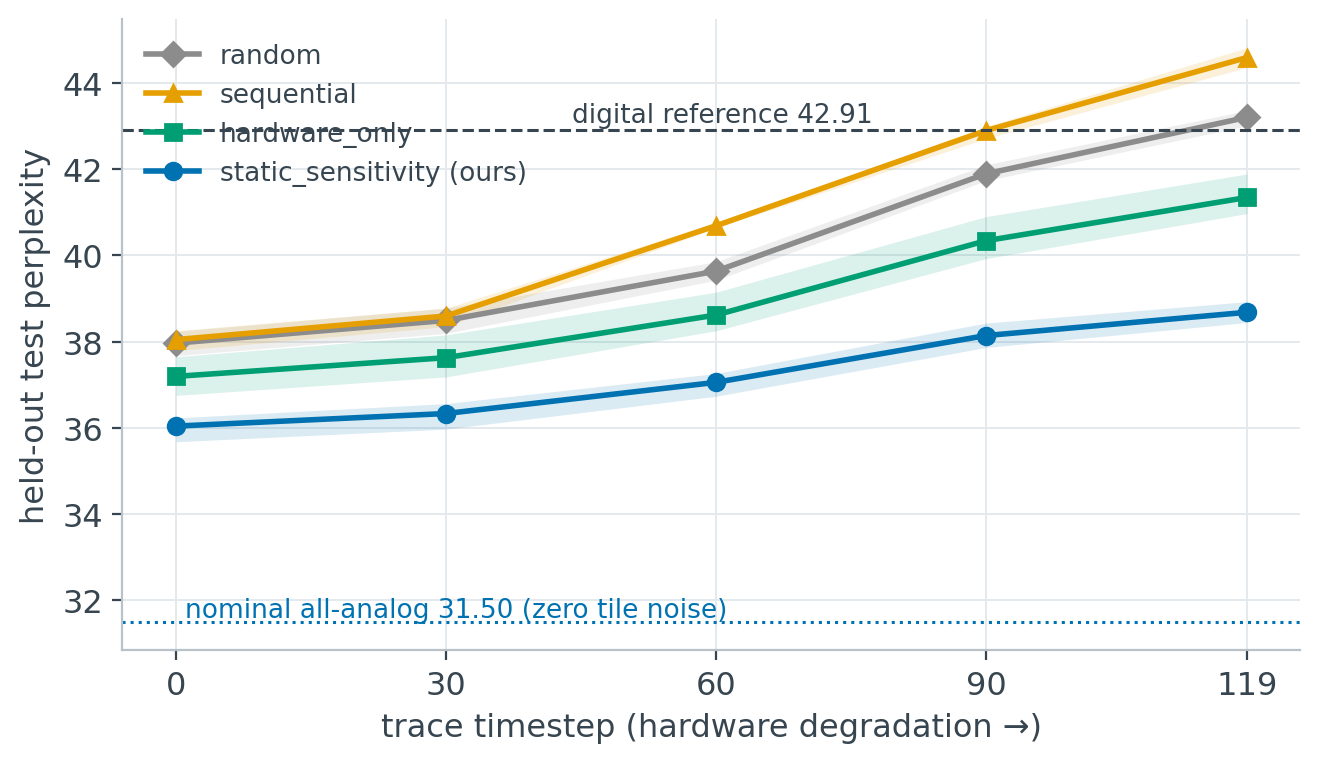
\includegraphics[width=0.80\columnwidth]{figures/p4_ppl.png}
\caption{Held-out test perplexity under the aging trace (trace 42; bands
= min/max over three paired realizations). Only sensitivity-aware
placement stays below the digital reference (dashed) throughout.}
\label{fig:ppl}
\end{figure}

\begin{table}[t]
\centering
\caption{End-of-life ($t{=}119$) test perplexity across five independent
hardware traces. Digital reference: $42.91$.}
\label{tab:eol}
\footnotesize
\begin{tabular}{lcccc}
\toprule
Policy & mean & std & worst cond. & above digital \\
\midrule
\policy{sequential} & 45.48 & 2.75 & 50.43 & 13/15 \\
\policy{random} & 45.38 & 1.84 & 48.05 & 15/15 \\
\policy{hardware\_only} & 42.82 & 1.61 & 45.90 & 6/15 \\
\policy{static\_sensitivity} & \textbf{39.30} & \textbf{0.60} &
\textbf{40.28} & \textbf{0/15} \\
\bottomrule
\end{tabular}
\end{table}

\subsection{Placement Wins, and the Edge Grows with Age}
\label{sec:r2}
Table~\ref{tab:paired} reports the paired improvement of
\policy{static\_sensitivity} over each baseline, aggregated across the
five traces. Every confidence interval excludes zero; all 75 paired
conditions favor the method against every baseline; the weakest trace
still improves by $+0.046$ nats over the strongest baseline. On the per-timestep trace (Fig.~\ref{fig:paired}) the
advantage over \policy{hardware\_only} doubles from $0.031$ to $0.067$
nats between $t{=}0$ and $t{=}119$, monotonically---sensitivity-aware
placement \emph{ages better}, because the shards that matter most sit on
the tiles that degrade least. Hardware awareness alone recovers roughly
half the benefit; knowing \emph{which shard matters} recovers the rest.
Placement also de-risks: end-of-life trace-to-trace spread is
$2.7$--$4.6\times$ smaller than the baselines' (Table~\ref{tab:eol}).

\begin{table}[t]
\centering
\caption{Cross-trace paired improvement of \policy{static\_sensitivity}
in $\dnll$ (nats); five traces as statistical units.}
\label{tab:paired}
\footnotesize
\begin{tabular}{lccc}
\toprule
Baseline & mean & 95\% t-CI & traces won \\
\midrule
\policy{hardware\_only} & $+0.063$ & $[0.042, 0.084]$ & 5/5 \\
\policy{random} & $+0.107$ & $[0.067, 0.147]$ & 5/5 \\
\policy{sequential} & $+0.106$ & $[0.048, 0.164]$ & 5/5 \\
\bottomrule
\end{tabular}
\end{table}

\begin{figure}[t]
\centering
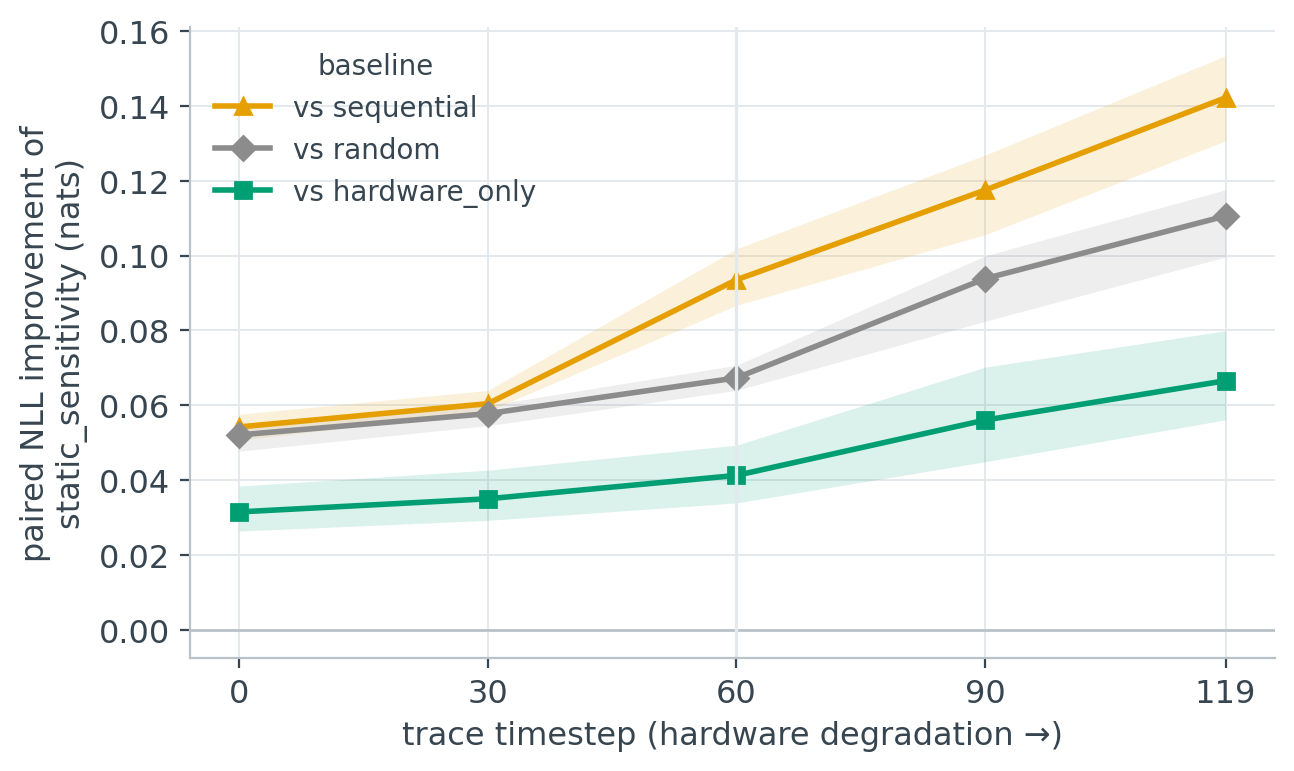
\includegraphics[width=0.80\columnwidth]{figures/p4_paired.png}
\caption{Per-timestep paired improvement of sensitivity-aware placement
(trace 42; bands = min/max over paired realizations). The advantage
grows monotonically as the hardware degrades.}
\label{fig:paired}
\end{figure}

\subsection{One-Shot Placement Is Near-Oracle}
\label{sec:r3}
Table~\ref{tab:bounds} adds the two bounding placements, evaluated on
the same five traces with exactly paired noise.
\policy{static\_sensitivity} captures $97.8\%$ of the
random$\rightarrow$clairvoyant headroom ($99.3\%$ of the full
adversarial-to-clairvoyant span); its residual gap to the clairvoyant
reference is $0.0024$ nats with a 95\% t-CI of $[-0.003, +0.008]$
across traces---at most an eighth of the headline effect,
\emph{statistically indistinguishable from zero}. Knowing the future buys
essentially nothing, bounding the value of adaptive remapping:
importance weighting already parks only low-importance shards on
fault-prone capacity, so faults arrive pre-mitigated. (The clairvoyant is $\Phi$-optimal under trajectory-RMS noise, not
NLL-optimal---hence \emph{reference}, not bound.) The adversarial edge of the
span: identical hardware, worst assignment, and the deployment sits
$1.8\times$ as far from nominal as \policy{random}, above the digital reference already at $t{=}0$
($45$--$47$ PPL, reaching ${\approx}59$ by end of life). Placement
spans working-versus-broken.

\begin{table}[t]
\centering
\caption{Placement span: mean $\dnll_{\mathrm{tile}}$ (nats) over all
timesteps, realizations, and five traces.}
\label{tab:bounds}
\footnotesize
\begin{tabular}{lcl}
\toprule
Placement & mean $\dnll_{\mathrm{tile}}$ & role \\
\midrule
\policy{adversarial} & 0.501 & worst-case bound \\
\policy{random} & 0.281 & baseline \\
\policy{sequential} & 0.280 & baseline \\
\policy{hardware\_only} & 0.236 & strongest baseline \\
\policy{static\_sensitivity} & \textbf{0.173} & proposed \\
\policy{oracle\_clairvoyant} & 0.171 & clairvoyant reference \\
\bottomrule
\end{tabular}
\end{table}

\subsection{Robustness Across Hardware Scenarios}
\label{sec:sweep}
Because the Phase-2 parameters are scenario values, we vary them one
factor at a time around the frozen configuration: fault count
($4/16$ tiles), drift range ($0.25$--$0.60$), thermal correlation
($\rho{=}0.7$), and tile-quality spread (mild $0.8$--$1.3\times$;
harsh $0.5$--$2.2\times$); one trace each,
$t \in \{0, 119\} \times 2$ realizations. The paired improvement is
positive in \textbf{48/48} conditions (6 variants $\times$ 2 baselines
$\times$ 2 timesteps $\times$ 2 realizations) and scales monotonically with
tile-quality spread---from $+0.027$ nats (mild) to $+0.073$ (harsh)
against the strongest baseline, a $2.7\times$ swing
(Table~\ref{tab:sweep})---while \policy{static\_sensitivity} ends below the digital reference in
all six variants (worst case $41.7$ under doubled drift) and the
baselines cross above it in the harsher half (\policy{random} in
three variants, \policy{hardware\_only} in two). The conclusion does not inherit the scenario choices: the less uniform
the substrate, the more placement pays.

\begin{table}[t]
\centering
\caption{Scenario sweep: paired improvement (nats) and end-of-life
PPL of \policy{static\_sensitivity}; digital $= 42.91$.}
\label{tab:sweep}
\footnotesize
\setlength{\tabcolsep}{4pt}
\begin{tabular}{lccc}
\toprule
Variant & vs \policy{hw\_only} & vs \policy{random} & EOL PPL \\
\midrule
spread\_low ($0.8$--$1.3\times$) & $+0.027$ & $+0.043$ & 39.80 \\
faults\_low (4 tiles) & $+0.042$ & $+0.073$ & 38.83 \\
thermal\_low ($\rho{=}0.7$) & $+0.052$ & $+0.075$ & 38.71 \\
faults\_high (16 tiles) & $+0.066$ & $+0.095$ & 39.56 \\
drift\_high ($0.25$--$0.60$) & $+0.068$ & $+0.106$ & 41.69 \\
spread\_high ($0.5$--$2.2\times$) & $+0.073$ & $+0.123$ & 38.85 \\
\bottomrule
\end{tabular}
\end{table}

% -------------------------------------------------------------------------
\section{Discussion and Limitations}
This study answers, for a fully analog decoder LLM, the two questions
left open in~\cite{lammie2026}: static mappings \emph{are} invalidated
by degradation---but only workload-blind ones---and intra-analog
tile-quality differences are the resource placement exploits, at zero
runtime cost.

Deliberate boundaries: simulation only, under a documented contract;
tile-level noise; fixed substrate geometry (tile/tier counts, the
${\sim}13\%$ spare margin); uniform within-projection sensitivity; dimensionless
timesteps (drift a phenomenological surrogate)---claims concern policy
ordering and mechanism, not calendar lifetime; energy and latency are
not modeled. Natural next steps: a device-calibrated companion
scenario using AIHWKit's PCM model; a GPT-2 Medium scale-generality study
(configuration prepared); drop-in integration with circuit-level
frameworks (DNN+NeuroSim~\cite{neurosim}) to co-report energy, latency,
and area; and composition with read-out compensation such as
AIDX~\cite{aidx}, which acts on \emph{how} weights are read, not
\emph{where} they are placed.

The tile-quality map corresponds to write-verify statistics gathered
during programming; GPT-2's pre-norm decoder is structurally
representative of the GPT family, so the mapper's inputs and mechanism
carry over to larger models.

\emph{Reproducibility:} code and configurations:
\url{https://github.com/williamhwangweiju/projection-sensitivity-mapping};
every reported number traces to a committed configuration file.

% -------------------------------------------------------------------------
\section{Conclusion}
For an all-analog GPT-2 on heterogeneous, aging in-memory compute tiles,
placement---free at map time---decides whether the deployment stays
better than digital over its lifetime. A measured projection-sensitivity profile
turns that decision from a risk into a near-oracle guarantee: $+0.063$ nats over the
strongest baseline (95\% t-CI $[0.042, 0.084]$, 5/5 traces), below-digital
quality in 75/75 lifetime conditions, 97.8\% of achievable headroom
captured, and robustness across all tested scenarios.

% -------------------------------------------------------------------------

\begin{thebibliography}{16}
\footnotesize

\bibitem{joshi2020}
V.~Joshi \emph{et al.}, ``Accurate deep neural network inference using
computational phase-change memory,'' \emph{Nat. Commun.}, vol.~11, 2020.

\bibitem{rasch2023}
M.~J. Rasch \emph{et al.}, ``Hardware-aware training for large-scale and
diverse deep learning inference workloads using in-memory
computing-based accelerators,'' \emph{Nat. Commun.}, vol.~14, 2023.

\bibitem{legallo2018}
M.~Le~Gallo \emph{et al.}, ``Mixed-precision in-memory computing,''
\emph{Nat. Electron.}, vol.~1, 2018.

\bibitem{wan2022}
W.~Wan \emph{et al.}, ``A compute-in-memory chip based on resistive
random-access memory,'' \emph{Nature}, vol.~608, 2022.

\bibitem{gpt2}
A.~Radford \emph{et al.}, ``Language models are unsupervised multitask
learners,'' OpenAI, 2019.

\bibitem{aihwkit}
M.~J. Rasch \emph{et al.}, ``A flexible and fast PyTorch toolkit for
simulating training and inference on analog crossbar arrays,'' in
\emph{Proc. IEEE AICAS}, 2021.

\bibitem{legallo2023}
M.~Le~Gallo \emph{et al.}, ``Using the IBM analog in-memory hardware
acceleration kit for neural network training and inference,''
\emph{APL Mach. Learn.}, vol.~1, 2023.

\bibitem{wikitext}
S.~Merity \emph{et al.}, ``Pointer sentinel mixture models,'' in
\emph{Proc. ICLR}, 2017.

\bibitem{ste}
Y.~Bengio \emph{et al.}, ``Estimating or propagating gradients through
stochastic neurons for conditional computation,'' arXiv:1308.3432, 2013.

\bibitem{lammie2026}
C.~Lammie, ``Heterogeneous mapping for analog in-memory computing
accelerators: A unified workflow,'' \emph{IEEE Comput. Archit. Lett.},
2026.

\bibitem{lionheart}
C.~Lammie \emph{et al.}, ``LionHeart: A layer-based mapping framework
for heterogeneous systems with analog in-memory computing tiles,''
\emph{IEEE Trans. Emerg. Topics Comput.}, 2025.

\bibitem{mps}
H.~Benmeziane \emph{et al.}, ``Supernetwork-based efficient mapping of
deep learning applications to mixed-precision hardware using model
adaptation,'' \emph{Nat. Commun.}, 2026.

\bibitem{xia2018}
L.~Xia \emph{et al.}, ``Stuck-at fault tolerance in RRAM computing
systems,'' \emph{IEEE JETCAS}, vol.~8, no.~1, 2018.

\bibitem{zhang2019}
B.~Zhang \emph{et al.}, ``Handling stuck-at-faults in memristor crossbar
arrays using matrix transformations,'' in \emph{Proc. ASP-DAC}, 2019.

\bibitem{neurosim}
X.~Peng \emph{et al.}, ``DNN+NeuroSim: An end-to-end benchmarking
framework for compute-in-memory accelerators with versatile device
technologies,'' in \emph{Proc. IEDM}, 2019.

\bibitem{aidx}
T.~Liu \emph{et al.}, ``AIDX: Adaptive inference scheme to mitigate
state-drift in memristive VMM accelerators,'' \emph{IEEE Trans.
Circuits Syst. II}, vol.~68, no.~4, 2021.

\end{thebibliography}

\end{document}
